\documentclass[../main.tex]{subfiles}

\graphicspath{{../images/}}

\begin{document}
\pagestyle{fancy}
\lhead{Lecture 8: 2/8}
\chead{Chapter 6}
\rhead{PHYS 472}

\section*{Chapter 6: Free Electron Fermi Gas}
\addcontentsline{toc}{section}{Chapter 6: Free Electron Fermi Gas}

Read
\href{https://en.wikipedia.org/wiki/Slater_determinant}{Slater Determinant}:
We typically use an approximation of the wavefunction for $N$ fermions as
\begin{align*}
    E\psi_N = \qt[\frac{-\hbar}{2m} \laplacian + V(\vb{r})] \psi_N
\end{align*}
found using the \href{https://en.wikipedia.org/wiki/Hartree%E2%80%93Fock_method}{Hartree-Fock method}
where we use the Slater determinant to find the energy of the system. For a system of $N$ fermions
we have a periodic potential and we can approximate this $N$ fermions to one mean-field. Also 
related: \href{https://en.wikipedia.org/wiki/Schwinger%E2%80%93Dyson_equation}{Dyson Equation}. When
we treat the group of particles as one \emph{mean-field} we call them \emph{quasiparticles}. The 
quasiparticle must obey the charge conservation e.g. a bare electron drags a positive cloud which
also drags nearby electrons as a quasi electron and the total charge of the dragged cloud is still
-1. We desire small mass quasi particles for semiconductors due to a faster acceleration. For the
free-electron case we assume that the electrons do not interact with each other thus, we can 
quanitize the single electron states.

\paragraph*{Energy} The quantized energies are related to the quantized standing waves of the 
particle in a box. The Hamiltonian is
\begin{align*}
    -\frac{\hbar^2}{2m} \dv[2]{x} \psi_n = E_n \psi_n
\end{align*}
which has a sinosoidal solution of the wavefunction
\begin{align*}
    \psi_n = A \sin(\frac{2\pi}{\lambda_n} x) 
\end{align*}
and the boundary condition determines the wavelength
\begin{align*}
    n \lambda_n = 2L
\end{align*}
and thus the energy of a state is
\begin{align*}
    E_n = \frac{\hbar^2 k^2}{2m} = \frac{\hbar^2}{2m} \qt(\frac{n\pi}{L})^2
\end{align*}

\paragraph*{Fermi (level) energy} is pretty much the highest occupied state (energy). For the 1D 
case the wave number can only be satisfied at the states for the standing waves:
\begin{align*}
    k_0 = 0, \quad k_2 = \pm \frac{2\pi}{L}, \quad k_4 = \pm \frac{4\pi}{L}, \quad \dots
\end{align*}
the fermi level at $N$ is
\begin{align*}
    k = \frac{N\pi}{2L} \to \epsilon_f = \frac{\hbar^2}{2m} \qt(\frac{N\pi}{2L})^2
\end{align*}

For the 3D case, we have a cube with a small box of volume $(\qt\frac{2\pi}{L}^3)$ and for the
large number $10^{23}$ we get a rough estimate of a spherical shell. The fermi energy is
\begin{align*}
    \frac{\frac{4}{3} \pi k_f^3}{\qt(\frac{2\pi}{L})^3} = \frac{N}{2}
\end{align*}
where the $N/2$ comes from the denegeracy of the spin states. This is equivalent to the ratio of the
volume of the sphere to the volume element. The fermi momentum is
\begin{align*}
    k_f = \qt(\frac{3}{8} \sqrt{(2\pi)^3}{L^3} \frac{1}{\pi})^{1/3}
\end{align*}
or 
\begin{align*}
    K_f = \qt(\frac{3\pi^2N}{V})^{1/3}
\end{align*}
and the fermi energy is
\begin{align*}
    \epsilon_f = \frac{\hbar^2}{2m} k_f^2 
    = \frac{\hbar^2}{2m} \qt(\frac{3\pi^2N}{V})^{2/3}
\end{align*}
and the electron velocity is
\begin{align*}
    v_f = \frac{\hbar k_f}{m} = \frac{\hbar}{m} \qt(\frac{3\pi^2N}{V})^{1/3}
\end{align*}
much like the phonon example, we can find the density of states for the free electron gas:
\begin{align*}
    D(\epsilon) = \dv{N}{\epsilon}
\end{align*}
we can solve the fermi energy equation as a function of energy
\begin{align*}
    N = \qt(\frac{2\epsilon m}{\hbar^2})^{3/2} \frac{V}{3\pi^2}
\end{align*}
we also have a relation between $N$ and $k_f$ so we can write the volume in $k$ space:
\begin{align*}
    V_k = \frac{4}{3} \pi k^3
\end{align*}
and since the energy is quantized as
\begin{align*}
    E = \frac{\hbar^2 k^2}{2m} \to k = \frac{\sqrt{2mE}}{\hbar}
\end{align*}
thus
\begin{align*}
    V_k = \frac{4}{3} \pi \frac{(2mE)^{3/2}}{\hbar^3}
\end{align*}
and since the number of states is
\begin{align*}
    N = \frac{V_k}{\qt(\frac{2\pi}{L})^3} \cdot 2 \\
    = \frac{V}{3\pi^2} \qt(\frac{2mE}{\hbar^2})^{3/2}
\end{align*}
thus the density of states is
\begin{align*}
    D(\epsilon) = \dv{N}{\epsilon} = \frac{V}{2\pi^2} \qt(\frac{2m}{\hbar^2})^{3/2} \sqrt{E}
\end{align*}
so the DOS is proportional to $\sqrt{E}$. Also it is proportional to the mass!


\newpage
\lhead{Lecture 9: 2/13}

\section*{Chapter 6: Cont'd}

\paragraph*{Fermi Energy} We have a 3D free electron gas with a DOS of
\begin{align*}
    D(\epsilon) = \square \epsilon^{1/2}
\end{align*}
For the 2D case we have 
\begin{align*}
    D(\epsilon) = const
\end{align*}
which will look like a Heaviside step function. For the 1D case we have
\begin{align*}
    D(\epsilon) = \frac{1}{\sqrt{\epsilon}}
\end{align*}
where we have the energy dispersion relation
\begin{align*}
    \epsilon = \frac{\hbar^2 k^2}{2m}
\end{align*}
for graphene (2D material) what does the DOS look like? We would expect it to look like step
function, but the electron dispersion relation is linear: $\epsilon = c k$ so the DOS is 
a linear function.
\paragraph*{weird li yang writing:}
\begin{align*}
    C_v \propto \alpha T^3 + \beta T
\end{align*}

\paragraph*{Fermi sphere}
\begin{figure}[ht]
    \centering
    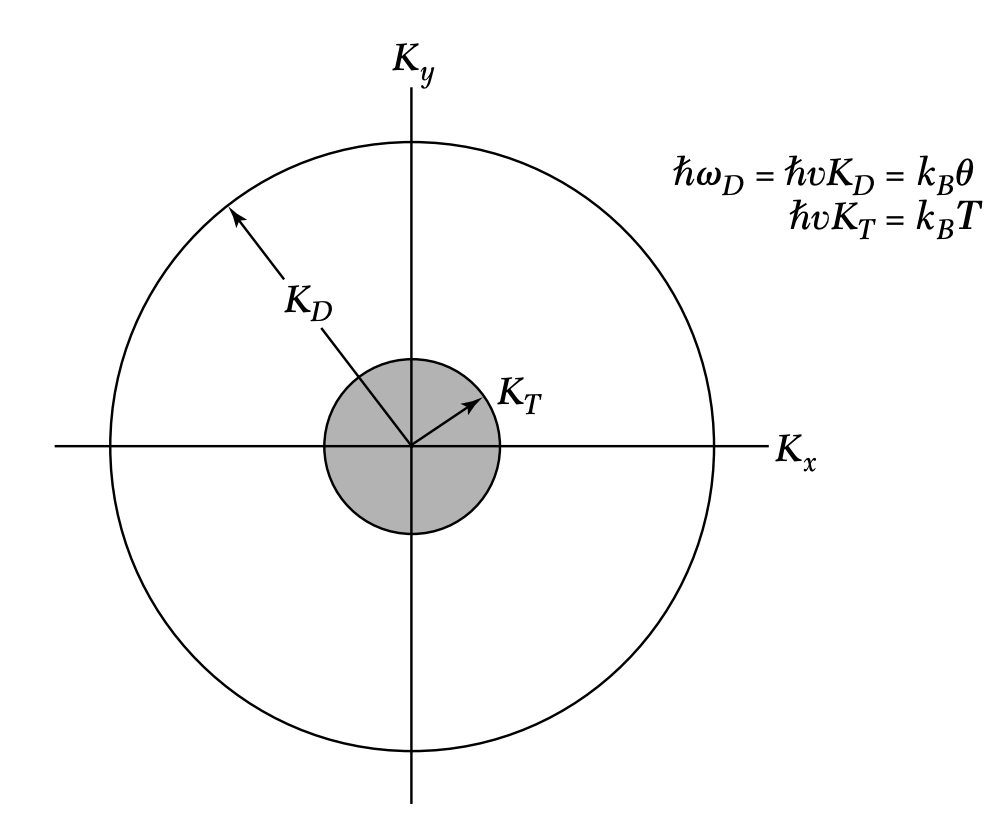
\includegraphics[width=0.4\linewidth]{debyelaw.png}
    \caption{Fermi sphere}
    \label{fig:6.1}
\end{figure}
at roughly 30 K the classical thermal energy is roughly $k_B T \sim 3$ meV. As the temperature goes
up, there is a smearing of the shell at the edges of the fermi sphere. So there are more electrons
that can be excited to hgiher energy states thus $N \propto k_B T$. The fermi energy is then roughly
$N k_B T \approx T^2 \propto U$. And the heat capacity is
\begin{align*}
    C_v \propto \pdv{U}{T} \propto T
\end{align*}

\paragraph*{Fermi-Dirac distribution} We have 3 parameters that describe the distribution
\begin{align*}
    f(T, \epsilon, \mu) = \frac{1}{\exp(\frac{\epsilon - \mu}{k_B T}) + 1}
\end{align*}
For $T\to 0$, if $\epsilon > \mu$ then $f \to 0$ and if $\epsilon < \mu$ then $f \to 1$. 
\begin{figure}[ht]
    \centering
    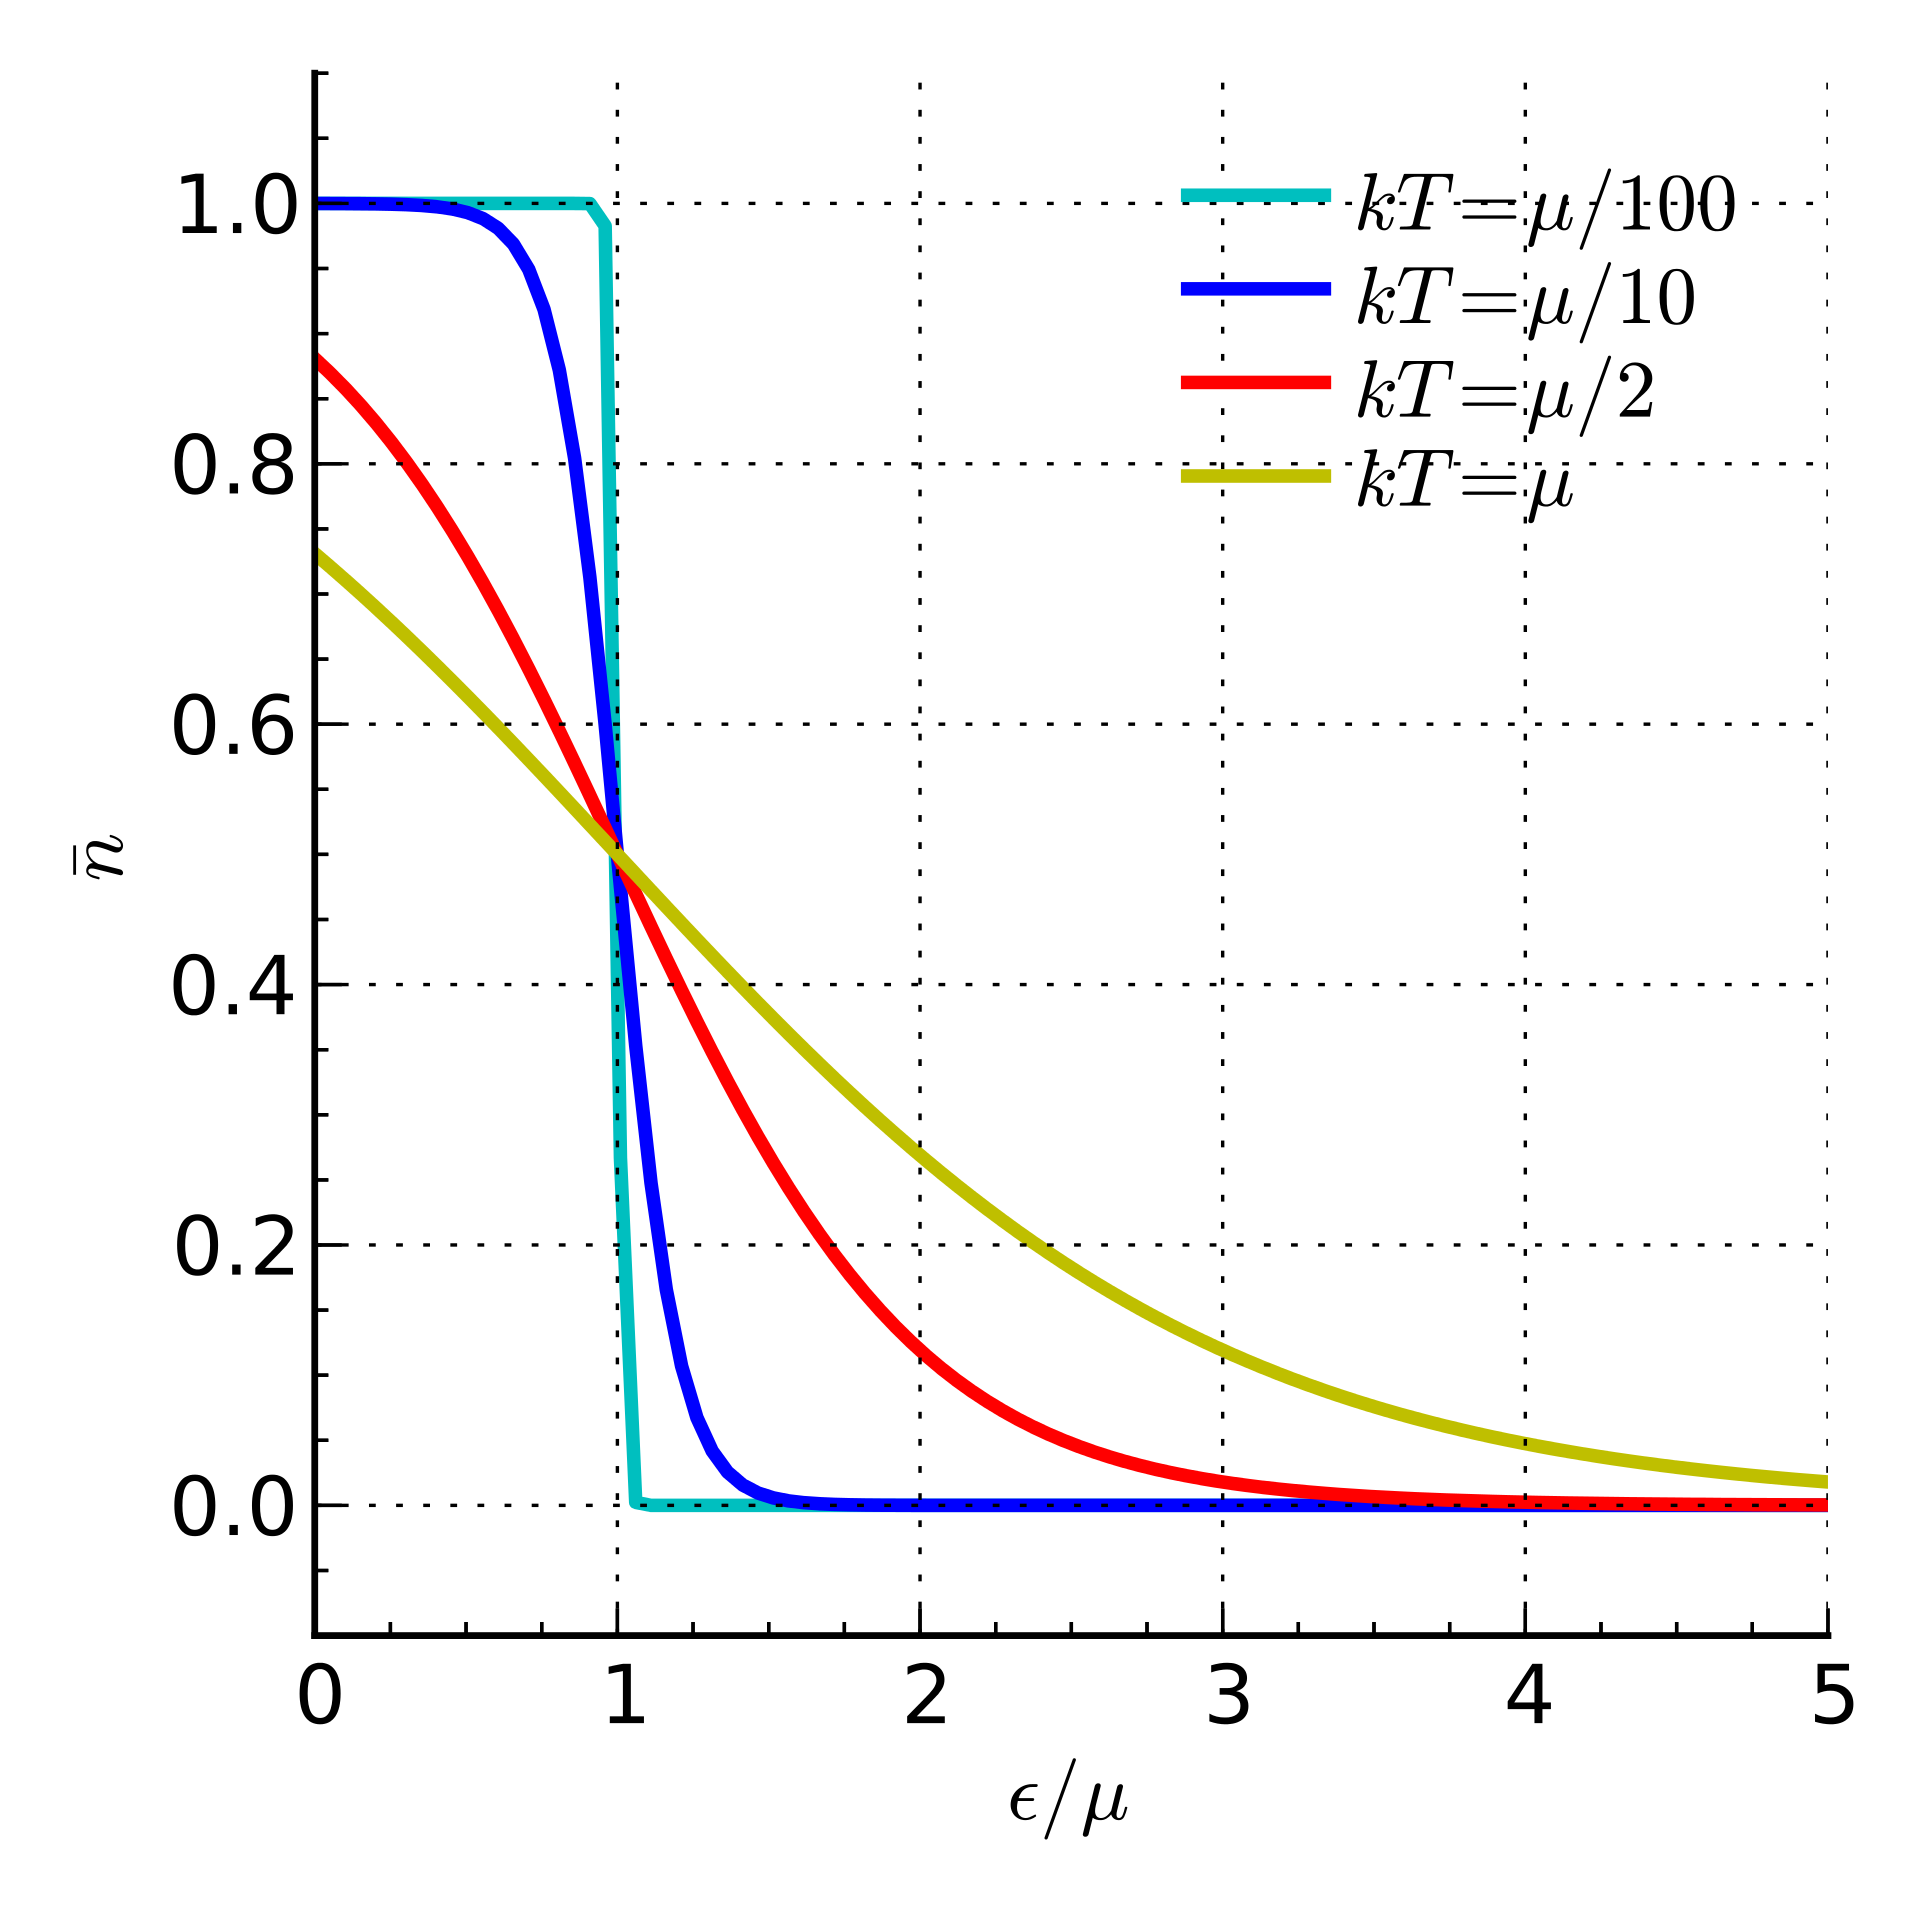
\includegraphics[width=0.4\linewidth]{fermi_dirac_dist.png}
    \caption{Fermi-Dirac distribution}
    \label{fig:6.2}
\end{figure}
at very small temperatures, we have a step function. As $T$ increases, the energy states
are more smoothed out.

\paragraph*{Energy change}
\begin{align*}
    \Delta U = U(T) - U(0)
\end{align*}
for $U(0)$ we have
\begin{align*}
    U(0) = \int_0^{\epsilon_f} \dd{\epsilon} D(\epsilon) \epsilon
\end{align*}
where we are taking the density of energy and multiplying by the energy at each state and summing 
them up from $0$ to $\epsilon_f$. For $U(T)$ we have
\begin{align*}
    U(T) &= \int_0^{\infty} \dd{\epsilon} D(\epsilon) \epsilon f(\epsilon) \\
    &= \qt(\int_0^{\epsilon_f} + \int_{\epsilon_f}^{\infty})
        \dd{\epsilon} D(\epsilon) \epsilon f(\epsilon)
\end{align*}
where we can split this integral into two parts. So we get the change in energy
\begin{align*}
    \Delta U &= \int_{\epsilon_f}^{\infty} [\epsilon - \epsilon_f] f(\epsilon) D(\epsilon) \dd{\epsilon} 
    + \int_0^{\epsilon_f} [\epsilon_f - \epsilon] [1 - f(\epsilon)] D(\epsilon) \dd{\epsilon}
\end{align*}
where the first term $I$ is the part to the right of the chemical potential and the second term $II$
is the part to the left of the chemical potential. We can then find the chemical potential in 
reference to the zero energy state.:
\begin{align*}
    C_v = \dv{(\Delta U)}{T} = \int_{\epsilon_f}^\infty \dd{\epsilon} 
    (\epsilon - \epsilon_f) \pdv{f}{T} D(\epsilon) + \int_0^{\epsilon_f} \dd{\epsilon} 
    (\epsilon_f - \epsilon) \qt(-\pdv{f}{T}) D(\epsilon) \\
    = \int_0^\infty \dd{\epsilon} (\epsilon - \epsilon_f) \pdv{f}{T} D(\epsilon)
\end{align*}
where we first redefine $\tau = k_B T$, and 
\begin{align*}
    f(\epsilon, \tau, \mu) = \frac{1}{\exp(\frac{\epsilon - \mu}{\tau}) + 1}
\end{align*}
so 
\begin{align*}
    \pdv{f}{T} = k_B \pdv{f}{\tau} = \frac{\epsilon - \epsilon_f}{\tau^2} 
        \frac{\exp(\frac{\epsilon - \mu}{\tau})}{(\exp(\frac{\epsilon - \mu}{\tau}) + 1)^2}
\end{align*}
as $\mu to \epsilon_f$. We can define another variable
\begin{align*}
    x = \frac{\epsilon - \mu}{\tau}
\end{align*}
So
\begin{align*}
    C_v = k_B^2 T D(\epsilon_f) \int_{-\epsilon_f/\tau}^\infty \dd{x} x^2 \frac{\exp(x)}{(\exp(x) + 1)^2}
\end{align*}
and at $T \to 0$ we get reduce this to
\begin{align*}
    C_v = k_B^2 T D(\epsilon_f) \int_{-\infty}^\infty \dd{x} x^2 \frac{\exp(x)}{(\exp(x) + 1)^2}
\end{align*}
and the analytical solution gives us
\begin{align*}
    \frac{\pi^2}{3}
\end{align*}
e.g. for the free electron gas with a DOS
\begin{align*}
    D(\epsilon_f) = \frac{3N}{2k_B T_f} 
\end{align*}
the heat capacity is
\begin{align*}
    C_v = \frac{1}{2} \pi^2 N k_B \frac{T}{T_f}
\end{align*}

\paragraph*{Electrical Conductivity}
for an electron the force is
\begin{align*}
    \vb{F} = -e \vb{E} = m \dv{\vb{v}}{t} = \hbar \dv{\vb{k}}{t} \\
    m \dv{\vb{v}}{t} = -e E \qquad \Delta U = -\frac{eE}{m} \Delta t
\end{align*}
From the Drude model, we have a mean free path that explains the motion of the electrons. This
$\Delta t$ is related to teh scattering (where high $\tau$ means less scattering). And from the
Drude model we can define the current density:
\begin{align*}
    \vb{j} = n e \vb{v} = n \frac{e^2 \tau \vb{E}}{m}
\end{align*}
with conductance
\begin{align*}
    \sigma = \frac{ne^2 \tau}{m}
\end{align*}
the overall collision time is 
\begin{align*}
    \frac{1}{\tau} = \frac{1}{\tau_1} + \frac{1}{\tau_2} + \dots
\end{align*}
So applying an electric field will shift the center of the fermi sphere since the electric field 
will apply a force on the electrons. 







\newpage
\lhead{Lecture 10: 2/15}

\section*{Chapter 6: Cont'd}
From the conductance eq, we usually see that well conductive materials have a lighter effective
mass. 

\paragraph*{Hall Effect:} Consider a 2D material with a longitudinal electric field $E_x$ and a
orthogonal magnetic field $\vb{H} = B_z$. There will be a resulting voltage drop(electric field) in
the transverse direction $E_y$: We first define the longitudinal conductance
\begin{align*}
    \rho(H) = \frac{E_x}{J_x}
\end{align*}
and the Hall coefficient is
\begin{align*}
    R_H = \frac{E_y}{J_x H}
\end{align*}
from the Lorentz force we have
\begin{align*}
    \dv{\vb p}{t} = q(\vb E + \frac{\vb p}{m} \times \vb H) - \frac{\vb p}{\tau}
\end{align*}
where $\vb p$ is the momentum. We can assume that this is a steady state:
\begin{align*}
    \dv{\vb p}{t} = 0
\end{align*}
and we can a set of equations for the steady state:
\begin{align*}
    \begin{cases}
        0 = qE_x - \omega_c p_y - \frac{p_x}{\tau} \\
        0 = qE_y + \omega_c p_x - \frac{p_y}{\tau}
    \end{cases}
\end{align*}
where $\omega_c = \frac{qH}{mc}$ is the cyclotron frequency. Or in terms of the conductance and 
resistivity:
\begin{align*}
    \begin{cases}
        -\sigma_0 E_x = \omega_c \tau j_y + j_x \\
        -\sigma_0 E_y = -\omega_c \tau j_x + j_y
    \end{cases}
\end{align*}
and since $j_y = 0$ we get
\begin{align*}
    -\sigma_0 E_x = j_x; \qquad \sigma_0 = -\frac{j_x}{E_x}, \\
    -\sigma_0 E_y = -\omega_c \tau j_x; \quad E_y = \frac{\omega_c \tau}{\sigma_0} j_x
\end{align*}
substituing back into the Hall coefficient we get
\begin{align*}
    R_H = \frac{E_y}{j_x H} = \frac{\omega_c \tau}{\sigma_0 H} = \frac{q \tau}{m c \sigma_0}  \\
    \qusing \sigma_0 = n \frac{q^2 \tau}{m} \\
    R_H = \frac{1}{ncq}
\end{align*}

\end{document}